%!TEX root=../../autopilot.tex
\section{Network Bandwidth}
\label{sec:bandwidth}

\begin{margintable}[0cm]
\caption{Bandwidth Test Materials!!!!}
\label{tab:gpiomaterials}
\noindent\begin{tabularx}{\linewidth}{lX}%
\toprule
\textbf{Terminal} & my freaking macbook \\
\textbf{Router} & some shitty consumer one! \\
\textbf{Code} & It's out there! \\
\bottomrule
\end{tabularx}
\end{margintable}

To test Autopilot's bandwidth, we demonstrate yet another modality of use, using Autopilot's \href{https://docs.auto-pi-lot.com/en/v0.5.0/gui/menus.html#autopilot.gui.menus.tests.Bandwidth_Test}{\texttt{Bandwidth\_Test}} widget, an action available from the Terminal GUI's \texttt{tests} menu that corresponds to a callback "listen" method in the Pilot. This test requests that one or several\sidenote{Since the Raspberry Pi, rather than the receiving Terminal, is overwhelmingly more likely to be the bandwidth bottleneck, so more pis behave like a linear multiple of a single pi, we only test with one here.} pilots send messages at a range of selected frequencies and payload sizes back to the terminal. The messages pass through four networking objects en route: the stations and network nodes running the test for both the terminal and pilots (See Figure \ref{fig:datastreams}). 

The needs for streaming experimental data vary depending on what is being streamed. Electrophysiological data is an n-electrode length vector sampled at a rate of dozens to hundreds of kilohertz, so each individual message isn't very large but there are a lot of them. Video data is a width by height (and for color video, by channel) array that can be relatively large\sidenote{(1920 * 1080 * 3 * 8 bits) / 8 = \~6 megabytes per frame of a 1080p color video, which is why video is rarely streamed uncompressed}, but it is captured at dozens to hundreds of hertz. Different data streams also have different degrees of compressibility: noisy, quasirandom electrical signals compress relatively poorly, while the typical behavioral neuroscientist's video of an animal that takes up 1/10th of the frame against a white background can have compression ratios in the hundreds.

Autopilot tries to provide flexibility for streaming different data types by offering message batching and optional on-the-fly compression with \href{https://www.blosc.org/}{blosc}. The bounds on bandwidth are then the speed at which an array can be compressed and the rate at which messages of a given size can be sent. 

Autopilot's networking modules were able to send an "empty" (402 byte) message with headers describing the test but no payload at a maximum observed rate of 1,818Hz\sidenote{maximum average rate of 5000 messages for each of the equivalent empty message tests in the four conditions described below}. Approximately 15\% of the duration is spent in message serialization, as a "frozen" preserialized message can be sent at 2,100Hz, though we imagine the need to send the same message thousands of times is rare.

We tested four types of messages with nonzero array\sidenote{In all cases, float64 numpy arrays encoded in base64} payloads: since the entropy of an array determines how compressible it is, we sent random and all-zero arrays with and without compression. The random and all-zero arrays are the floor and ceiling of compressibility, respectively. Compression gives us two notions of bandwidth: the literal number of bytes that can be passed through a connection, and the effective bandwidth of the size of the arrays that can be transferred with a given compression ratio. We refer to these as "message" and "payload" bandwidth, respectively in Figure \ref{fig:bandwidth}. Message bandwidth reflects the hardware limitations of the Raspberry Pi, but payload bandwidth is the number that matters in practice, as it measures the actual "speed of data" that can be used by the receiver.

As we increased the size of the array payload\sidenote{n=5,000 for each condition at each size}, the message bandwidth plateaued at a maximum of 29.25MByte per second (Figure \ref{fig:bandwidth}, left). After this plateau, increasing the message size trades off linearly with the rate of messages sent. For all but the compressed array of zeros, the payload bandwidth mirrored the message bandwith with some trivial overhead from the base64 encoding. The compressed array of zeros, however, had an effective payload bandwidth of 169.6MBytes/s, a compromise between the speed of compression with the smaller message size\sidenote{A message with a \~1MByte zero array payload compressed to \~6KBytes.}. The compressed random array had only negligible differences in payload and message bandwidth compared to the uncompressed random array, indicating that the overhead for blosc is trivial. 

The ability to batch messages allows researchers to tune the size of an individual message to their particular need for high bandwidth or low latency. Since the compressibility of real data varies across the entire entropic range from randomness to arrays of all zeros, Autopilot doesn't have a single "bandwidth", but one that ranges between 30 and 170MByte/s\sidenote{In this dataset. There is additional payload bandwidth headroom with larger messages, and we include an additional dataset with a 200MByte/s bandwidth in the supplement.} 

\begin{figure}[t]
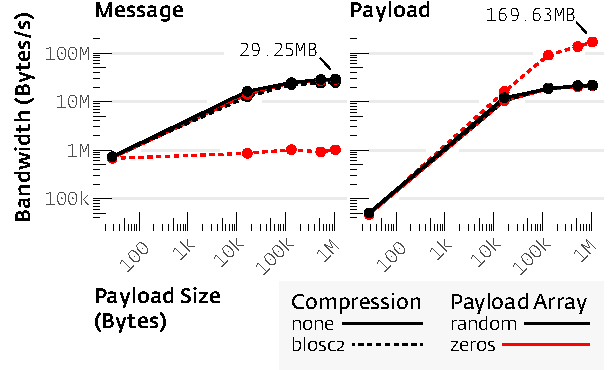
\includegraphics[]{figures/networking_bandwidth.pdf}
\caption{Bandwidth measurements between a pilot and terminal for compressed (solid lines) or uncompressed (dotted lines) arrays of random numbers (black) or zeros (red, each point n=5000 messages). As message size increased, the bandwidth for the rate of bytes transferred in serialized messages ("message bandwidth," left) plateaued at 29.25MBytes/s, while the effective bandwidth of arrays before and after compression ("payload bandwidth," right) reached 169.63MBytes/s. Real data will fall somewhere in this effective bandwidth range, depending on its compressibility.}
\label{fig:bandwidth}
\end{figure}

This bandwidth makes Autopilot capable of streaming raw Calcium imaging\sidenote{2-Photon:  5.9MB/s\\ \noindent (12 bits * 512x512 resolution * 15Hz)} and electrophysiological data from modern high-density probes\sidenote{Neuropixels: 14.4MB/s\citep{junFullyIntegratedSilicon2017}\\\noindent(10 bits * 30kHz * 384 channels)}. Its flexible architecture allows researchers to decide how to build their experiments by distributing different components over different combinations of computers: stream data from a raspberry pi to a more powerful computer for processing, use GPIO rather than network triggers for time-critical operations --- meeting the tooling challenge of complex, hardware-intensive, multimodal experiments that define contemporary systems neuroscience.